% ============================================================================
%  report1_asv_planner.tex
%  Comprehensive internship report -- ASV Positioning Planner for acoustic-aided
%  AUV localisation: the working system, its results, an analysis of the cost,
%  honest limitations, and full derivations.
%
%  Modern LaTeX (book class) -- compiles on Overleaf / current TeX.
%  FIGURES in ./figs/  : ASV_Planner_flowchart.png (block diagram),
%    Trajectory Generation.png, survey_geometry.png, results_traj2d.png,
%    results_asv_track.png, results_traj3d.png, infogain_vs_bearing.png.
%  BIBLIOGRAPHY: ref.bib (biblatex). Every ref.bib entry is flagged % VERIFY.
% ============================================================================
\documentclass[12pt,a4paper,oneside]{book}
\usepackage[utf8]{inputenc}
\usepackage[english]{babel}
\usepackage{lmodern}
\usepackage{amsmath}
\usepackage{amssymb}
\usepackage{graphicx}
\usepackage[top=1in, bottom=1in, left=1in, right=1in]{geometry}
\usepackage{float}
\usepackage[font={small}]{caption}
\usepackage{setspace}
\usepackage{booktabs}
\usepackage{array}
\usepackage[autostyle]{csquotes}
\usepackage[sorting=none]{biblatex}
\addbibresource{ref.bib}
\usepackage{hyperref}
\hypersetup{
  colorlinks = true,
  citecolor  = green,
  urlcolor   = blue,
  linkcolor  = black,
  pdfauthor  = {Minha Ansar},
  pdftitle   = {ASV Positioning Planner for Acoustic-Aided AUV Localisation},
  linktocpage
}

% ------------------------------- cross-ref macros ---------------------------
\newcommand{\eqnref}[1]{Eq.~(\ref{#1})}
\newcommand{\figref}[1]{Fig.~\ref{#1}}
\newcommand{\tabref}[1]{Table~\ref{#1}}
\newcommand{\secref}[1]{Sec.~\ref{#1}}
\newcommand{\chapref}[1]{Chapter~\ref{#1}}

% ------------------------------- title block --------------------------------
\title{
\sc
\Huge{An Adaptive Surface-Vehicle Positioning Planner}\\[8pt]
\Large{for Acoustic-Aided Localisation of}\\[4pt]
\Huge{Autonomous Underwater Vehicles}
\\[40pt]
\large{An Internship Project Report}
\\[5pt]
\normalsize{submitted in partial fulfilment of the requirements}
\\[5pt]
\normalsize{of the research internship}
\\[30pt]
\normalsize{by}
\\[15pt]
\large{Minha Ansar}
\\[5pt]
\normalsize{Indian Institute of Science}
\\[30pt]
\IfFileExists{figs/iisc_logo.jpg}{\includegraphics[scale=0.12]{figs/iisc_logo.jpg}\\[30pt]}{}
\normalsize{Under the supervision of}
\\[10pt]
\large{Prof.\ Suresh Sundaram}\\
\normalsize{Department of Aerospace Engineering}
\\[25pt]
\normalsize{August 2026}
}
\author{}
\date{}

\graphicspath{{figs/}}

\begin{document}
\singlespacing
\begin{titlepage}
\maketitle
\end{titlepage}
\onehalfspacing
\frontmatter
\setlength{\parskip}{5pt}

% ------------------------------- acknowledgements ---------------------------
\chapter*{\centering Acknowledgements}
\addcontentsline{toc}{chapter}{Acknowledgements}
\hspace{15pt}I express my sincere gratitude to Prof.\ Suresh Sundaram of the Department of Aerospace
Engineering, Indian Institute of Science, for hosting me in his research group during the period
covered by this report and for guiding the work documented here. I also thank the Department of
Aerospace Engineering at the Indian Institute of Science for providing access to compute resources and
laboratory infrastructure, and my colleagues at the Artificial Intelligence and Robotics Laboratory
(AIRL).

% ------------------------------- abstract -----------------------------------
\chapter*{\centering Abstract}
\addcontentsline{toc}{chapter}{Abstract}
\hspace{15pt}
Autonomous underwater vehicles (AUVs) navigate by dead reckoning on an inertial measurement unit (IMU);
with no satellite positioning underwater, this estimate drifts without bound. The only absolute correction
is an acoustic position fix delivered by an ultra-short-baseline (USBL) transceiver on a surface support
vehicle (an autonomous surface vehicle, ASV). Such fixes are slow and energy-costly, so they must be used
sparingly and delivered from a good relative geometry. This report describes a planner that decides
\emph{where the single ASV should position itself}, and \emph{when and which AUV it should ping}, so that a
fleet of surveying AUVs is kept within acoustic range and corrected before its uncertainty grows too large.
The ASV maintains a private, communication-free ``shadow'' estimate of each AUV's position and covariance,
triggers a fix when that covariance crosses a threshold, and steers using a sampling-based
Model-Predictive Path-Integral (MPPI) planner. In a two-AUV lawnmower survey simulation the planner keeps
both vehicles inside a 500\,m USBL envelope, delivers every requested fix with none lost, and holds the true
cross-track error near 2\,m throughout. For context, an unaided inertial navigator with the same class of
IMU exceeds a survey-grade budget within about twelve seconds, and periodic surfacing for GPS is shown to be
impractical at survey depth. The report also analyses the structure of the planner's cost, and documents an
open issue---a persistent low-amplitude wobble in the ASV's motion---together with the experiments that
localise its cause.

{\hypersetup{linkcolor=black} \tableofcontents}
{\hypersetup{linkcolor=black} \listoffigures}
{\hypersetup{linkcolor=black} \listoftables}

% ------------------------------- notation -----------------------------------
\chapter*{\centering Notation and Abbreviations}
\addcontentsline{toc}{chapter}{Notation and Abbreviations}
\begin{center}
\begin{tabular}{@{}ll@{}}
\toprule
Symbol / term & Meaning \\
\midrule
AUV & Autonomous Underwater Vehicle \\
ASV & Autonomous Surface Vehicle (the support / relay vehicle) \\
IMU & Inertial Measurement Unit (3-axis gyroscope + accelerometer) \\
USBL & Ultra-Short-Baseline acoustic positioning \\
EKF & Extended Kalman Filter \\
MPPI & Model-Predictive Path-Integral control \\
OOSM & Out-Of-Sequence Measurement \\
COG & Course-Over-Ground (heading aid) \\
$\mathbf{x},\,\mathbf{P}$ & EKF state estimate and covariance \\
$\mathbf{F},\,\mathbf{Q}$ & state-transition Jacobian and process-noise covariance \\
$\mathbf{H},\,\mathbf{R}$ & measurement Jacobian and measurement-noise covariance \\
$\mathbf{J}$ & measurement information matrix ($\mathbf{J}=\mathbf{R}^{-1}$) \\
$\Gamma$ & information gain (value of a candidate ping) \\
$\tau_{\text{trig}}$ & covariance trigger threshold \\
$D$-optimality & log-determinant information criterion \\
NEES / ANEES & (Average) Normalised Estimation Error Squared (consistency test) \\
\bottomrule
\end{tabular}
\end{center}

\mainmatter

% ============================================================================
\chapter{Introduction}
\label{ch:intro}

\section{Motivation}
An IMU reports linear acceleration and angular rate. Recovering position from it requires double
integration, so small sensor errors accumulate and the position estimate \emph{drifts without bound}. On
land or in the air this is corrected by GPS; underwater, radio does not propagate and no such signal
exists. The consequence is severe: as quantified in \chapref{ch:results}, an unaided inertial navigator
with a representative micro-electromechanical (MEMS) IMU sees its own position uncertainty cross a
survey-grade budget of $4.47$\,m within about \textbf{twelve seconds}, after which the estimate diverges to
kilometre scale and the survey can never be completed.

The solution is an \emph{acoustic} position fix. A surface vehicle carrying a USBL transceiver measures the
range and bearing to a submerged AUV, and hence its three-dimensional position, which is fed back into the
AUV's navigation filter to collapse the accumulated error. Acoustic fixes are, however, expensive: the
channel is half-duplex (one exchange at a time), each ping consumes energy, and the quality of the fix
depends on the relative geometry between the ASV and the AUV. A single ASV supporting several AUVs therefore
cannot ping continuously; it must \emph{position itself well} and \emph{choose its pings carefully}.

\section{Problem statement and objective}
This work develops the \emph{ASV positioning planner}: the decision layer that, at every planning slot,
(i) predicts where each AUV is and how uncertain that estimate has become, (ii) decides whether and which
AUV to ping, and (iii) steers the ASV to a position that keeps the fleet reachable and maximises the value
of the next fix. The design goal is to hold each AUV's position error under a survey-grade budget while
keeping the acoustic effort low and every requested fix deliverable.

\section{Contributions}
\begin{enumerate}
\item A \emph{communication-free} ASV-side model (a per-AUV ``shadow'') that reconstructs each AUV's
position and covariance from public information only, so the ASV can decide when a fix is due without any
acoustic uplink from the AUV (\secref{sec:shadow}).
\item A covariance-triggered fix mechanism with a three-tier scheduler that serves one AUV per acoustic slot
under the half-duplex constraint (\secref{sec:trigger}).
\item An information-driven MPPI positioning cost that trades the expected information of the next fix
($D$-optimality) against keeping the whole fleet within acoustic range (\secref{sec:mppi}).
\item A simulation study (\chapref{ch:results}), a structural analysis of the cost (\chapref{ch:analysis}),
and an honest account of an open issue in the ASV's motion (\chapref{ch:conclusion}).
\end{enumerate}

\section{Organisation}
\chapref{ch:background} reviews the background. \chapref{ch:model} gives the system model.
\chapref{ch:planner} presents the planner. \chapref{ch:setup} describes the simulation setup and metrics.
\chapref{ch:results} reports results, \chapref{ch:analysis} analyses the cost, and \chapref{ch:conclusion}
concludes with limitations and future work. Appendix~\ref{app:deriv} gives full derivations.

% ============================================================================
\chapter{Background and Related Work}
\label{ch:background}

\section{Underwater navigation and inertial drift}
Underwater vehicles cannot use GPS while submerged, so they rely on dead reckoning: integrating IMU
measurements to propagate position. Because position is the double integral of acceleration, biases and
noise in the IMU accumulate quadratically in time, and the estimate drifts without bound. Surveys of AUV
navigation and localisation \cite{kinsey2006survey,paull2014auv} catalogue the sensor suites and aiding
strategies used to contain this drift, from onboard aids (compass, DVL, pressure) to external acoustic
positioning.

\section{Acoustic positioning}
Acoustic positioning systems localise a submerged vehicle from the travel time and geometry of sound
pulses. In \emph{ultra-short-baseline} (USBL) positioning a single transceiver measures both the
\emph{range} to a transponder (from the two-way travel time) and the \emph{bearing} (from the phase
difference across a compact array of elements), yielding a three-dimensional relative position;
long-baseline (LBL) and short-baseline (SBL) systems instead triangulate from widely spaced elements.
Using such fixes to \emph{bound} the otherwise unbounded inertial drift is the central idea this work builds
on \cite{bindusbl}.

\section{Estimation and consistency}
The AUV's navigation is an extended Kalman filter (EKF). A key requirement is \emph{consistency}: the
filter's reported covariance must match its actual error statistics, or any decision that reads the
covariance (such as our fix trigger) acts on a lie. Consistency is checked with the normalised estimation
error squared (NEES), whose average (ANEES) should lie near unity for a well-tuned filter
\cite{barshalom2001estimation}.

\section{Sampling-based motion planning and information-driven sensing}
The ASV chooses its motion with Model-Predictive Path-Integral (MPPI) control, a sampling-based
model-predictive method that draws many random control sequences, evaluates a cost for each, and forms a
cost-weighted (softmax) average \cite{williams2017mppi}. The cost rewards \emph{information gain}: the
expected reduction in an AUV's position uncertainty from a fix taken at a candidate ASV location, scored by
the $D$-optimality (log-determinant) criterion from optimal experimental design. The marine vehicle
dynamics (the Otter surface craft and the REMUS-class AUV) follow standard models of marine-craft
hydrodynamics and motion control \cite{fossen2011handbook}.

% ============================================================================
\chapter{System Model}
\label{ch:model}

\section{Overview}
The system is a closed loop between two underwater AUV clients and one surface ASV (\figref{fig:block}).
Each AUV runs an inertial navigation filter and follows a preset lawnmower survey path. The ASV maintains,
for each AUV, a \emph{shadow} of its position and covariance; when a shadow's uncertainty crosses a
threshold the ASV pings that AUV over the USBL link, and the resulting three-dimensional fix collapses both
the AUV's own covariance and the ASV's shadow. Between pings the ASV continuously re-plans its motion so
that the fleet stays within acoustic range and the next fix has good geometry.

\begin{figure}[H]
\centering
\IfFileExists{ASV_Planner_flowchart.png}
  {\includegraphics[width=\linewidth]{ASV_Planner_flowchart.png}}
  {\framebox[0.9\textwidth]{\parbox{0.85\textwidth}{\centering\vspace{2cm}
   \textbf{[ place \texttt{figs/ASV\_Planner\_flowchart.png} ]}\vspace{2cm}}}}
\caption{Subsystem block diagram of the ASV positioning planner and its closed loop with the AUV clients
and the USBL acoustic link.}
\label{fig:block}
\end{figure}

The key architectural choice is that the ASV \emph{initiates everything}. There is no acoustic uplink in
which an AUV requests a fix: the ASV reconstructs each AUV's uncertainty on its own (from public information
only) and decides for itself when a correction is due.

\section{Walkthrough of the block diagram}
\label{sec:walkthrough}
\figref{fig:block} is a closed loop. The blocks are described below in signal-flow order, each as
input~$\to$~function~$\to$~output; the governing equations are given in the sections that follow and are
only cross-referenced here.

\paragraph{AUV client (the vehicle being served).}
\begin{description}
\item[IMU sensor.] In: the AUV's true motion. Function: measures three-axis angular rate and specific force
each tick (with bias and noise). Out: the gyro $\boldsymbol{\omega}$ and accelerometer $\mathbf{a}$
readings---the only proprioceptive information the submerged AUV has.
\item[EKF estimate.] In: the IMU stream, the sensor-free aids, and any USBL fix. Function: the $15$-state
inertial navigation filter (\secref{sec:usblmodel} and below) propagates on the IMU and corrects with the
aids and fixes. Out: the AUV's estimated state $\hat{\mathbf{x}}$ and covariance $\mathbf{P}$; between fixes
this estimate drifts.
\item[Lawn-mower reference.] In: the survey plan. Function: supplies the preset lawnmower waypoints
(parallel legs joined by turns) the AUV must follow. Out: the desired path fed to the guidance controller.
\item[Guidance controller.] In: the lawn-mower reference and the EKF \emph{estimate}. Function: an integral
line-of-sight path-follower that steers on the vehicle's own estimate (never truth), closing the AUV
guidance loop. Out: heading and depth commands to the AUV's actuators.
\end{description}

\paragraph{ASV positioning planner (one decision slot).}
\begin{description}
\item[AUV path predictor (shadow).] In: the AUV's last USBL fix and its publicly-known planned path.
Function: projects the AUV forward along the path and propagates a shadow covariance from public knowledge
only (\secref{sec:shadow}). Out: a predicted AUV position and covariance $\mathbf{P}$, per AUV.
\item[Ping decision.] In: each AUV's shadow-covariance trace and its time since last fix. Function: tests
$\operatorname{tr}(\mathbf{P}^{\text{pos}})>\tau_{\text{trig}}$ (\secref{sec:trigger}); on ``yes'' it selects
which AUV to ping, on ``no'' the slot passes with no fix (``no AUV position obtained''). Out: a ping target,
or none this slot.
\item[MPPI planner.] In: the per-AUV predicted position and covariance and the ASV's own pose. Function:
scores candidate ASV positions by the cost---information gain versus coverage versus control effort
(\secref{sec:mppi}). Out: a preferred committed control.
\item[Trajectory generation.] In: the sampled control rollouts. Function: rolls out $K$ candidate ASV paths
and forms their cost-weighted (softmax) average. Out: the committed reference---the first waypoint---handed
to the low-level controller.
\item[PD controller.] In: the committed reference and the ASV's pose. Function: a lookahead waypoint
follower with proportional--derivative steering. Out: the two Otter thruster commands $(f_L,f_R)$.
\item[ASV dynamics.] In: the thruster commands. Function: the Otter surface-vehicle dynamics. Out: the ASV's
new position, which feeds back to the planner and the low-level controller.
\end{description}

\paragraph{Acoustic link (closing the loop).}
\begin{description}
\item[USBL transceiver.] In: the ASV position and the ping target. Function: emits an interrogation pulse
and, from the transponder reply, measures range (round-trip time) and bearing (array phase)
(\secref{sec:usblmodel}). Out: a three-dimensional AUV position fix.
\item[Two-way exchange and fix.] In: the interrogation/reply pair. Function: the fix arrives after an
acoustic delay and is applied as an out-of-sequence measurement. Out: it collapses \emph{both} the AUV's EKF
covariance and the ASV's shadow, restarting the cycle.
\end{description}

\section{The AUV navigation filter}
Each AUV carries a $15$-state EKF with state vector
\begin{equation}
\mathbf{x} = \big[\,x,\,y,\,v_x,\,v_y,\,\psi,\,\phi,\,\theta,\;
b_{ax},\,b_{ay},\;b_{gx},\,b_{gy},\,b_{gz},\;z,\,v_z,\,b_{az}\,\big]^{\!\top} \in \mathbb{R}^{15},
\label{eq:state}
\end{equation}
comprising position $(x,y,z)$, velocity $(v_x,v_y,v_z)$, attitude (roll $\phi$, pitch $\theta$, yaw
$\psi$), gyroscope bias $(b_{gx},b_{gy},b_{gz})$ and accelerometer bias $(b_{ax},b_{ay},b_{az})$. The
initial covariance $\mathbf{P}_0$ and process-noise covariance $\mathbf{Q}$ are diagonal and derived from
the IMU specification (Appendix~\ref{app:params}).

\subsection{Prediction (strapdown propagation)}
Each tick the raw accelerations and yaw rate are de-biased and gravity is removed using the estimated
roll/pitch. Writing $c=\cos\psi$, $s=\sin\psi$, the de-biased horizontal accelerations
$a_x^c,a_y^c$ (and $a_z^c$, $r^c$ the de-biased yaw rate) are rotated into the world frame and integrated:
\begin{align}
a_x^w &= c\,a_x^c - s\,a_y^c, & a_y^w &= s\,a_x^c + c\,a_y^c, \label{eq:rot}\\
x &\mathrel{+}= v_x\,\Delta t + \tfrac12 a_x^w\,\Delta t^2, &
y &\mathrel{+}= v_y\,\Delta t + \tfrac12 a_y^w\,\Delta t^2, \label{eq:pos}\\
v_x &\leftarrow \lambda\,(v_x + a_x^w\,\Delta t), &
v_y &\leftarrow \lambda\,(v_y + a_y^w\,\Delta t), \label{eq:vel}\\
\psi &\leftarrow \operatorname{wrap}(\psi + r^c\,\Delta t), &
z &\mathrel{+}= v_z\,\Delta t + \tfrac12 a_z^c\,\Delta t^2, \label{eq:psiz}\\
v_z &\leftarrow \lambda\,(v_z + a_z^c\,\Delta t), \label{eq:vz}
\end{align}
where $\lambda$ is a small velocity-damping factor. The vertical channel carries no heading rotation, so
depth is decoupled from yaw. The covariance propagates as
\begin{equation}
\boxed{\;\mathbf{P} \leftarrow \mathbf{F}\,\mathbf{P}\,\mathbf{F}^{\!\top} + \mathbf{Q}\;},
\qquad \mathbf{F}=\frac{\partial \mathbf{x}^{+}}{\partial \mathbf{x}},
\label{eq:covprop}
\end{equation}
with the state-transition Jacobian $\mathbf{F}$ derived in Appendix~\ref{app:F}.

\subsection{Sensor-free attitude aids}
Two aids keep attitude observable without adding sensors. \emph{Gravity levelling} uses the fact that a
near-static accelerometer measures the direction of gravity, giving a soft measurement of roll and pitch on
the quasi-static survey legs. The \emph{course-over-ground} (COG) heading aid asserts that the heading
equals the direction of travel when side-slip is small, i.e.\ it drives the residual
\begin{equation}
c_{\text{cog}}(\mathbf{x}) = \psi - \operatorname{atan2}(v_y,\,v_x)
\label{eq:cog}
\end{equation}
toward zero with a soft measurement (Jacobian in Appendix~\ref{app:F}), gated on sufficient speed and low
turn rate. COG makes yaw observable from motion alone, which is essential on the long straight legs where
yaw is otherwise the weakest axis.

\subsection{USBL update and out-of-sequence handling}
A USBL fix is an absolute three-dimensional position measurement $\mathbf{z}=[n_x,n_y,n_z]^{\top}$ fused
with the standard EKF update (derived in Appendix~\ref{app:upd})
\begin{equation}
\boldsymbol{\nu}=\mathbf{z}-\mathbf{H}\mathbf{x},\quad
\mathbf{S}=\mathbf{H}\mathbf{P}\mathbf{H}^{\!\top}+\mathbf{R},\quad
\mathbf{K}=\mathbf{P}\mathbf{H}^{\!\top}\mathbf{S}^{-1},\quad
\mathbf{x}\leftarrow\mathbf{x}+\mathbf{K}\boldsymbol{\nu},\quad
\mathbf{P}\leftarrow(\mathbf{I}-\mathbf{K}\mathbf{H})\mathbf{P},
\label{eq:usblupdate}
\end{equation}
where $\mathbf{H}$ selects the three position states. Because sound is slow, the fix corresponds to a moment
in the past; it is applied as an \emph{out-of-sequence measurement} (OOSM), detailed in
Appendix~\ref{app:oosm}: the filter keeps a short history of $(t,\mathbf{x},\mathbf{P},\text{IMU})$, rewinds
to the entry nearest the fix's valid time, fuses \eqnref{eq:usblupdate} there, and replays the stored IMU
forward to the present.

\section{The USBL measurement model}
\label{sec:usblmodel}
The information a fix carries depends on the ASV--AUV geometry. For slant range $sl$ and bearing $brg$ the
measurement is precise along the range direction and coarse across it (the angular error grows with range).
The $2\times2$ horizontal measurement information matrix (derived in Appendix~\ref{app:J}) is
\begin{equation}
\mathbf{V}=\begin{bmatrix}\cos brg & -\sin brg\\ \sin brg & \cos brg\end{bmatrix},\quad
\boldsymbol{\Lambda}=\operatorname{diag}(\sigma_r^2,\;\sigma_{\text{ang}}^2),\quad
\mathbf{R}_m=\mathbf{V}\boldsymbol{\Lambda}\mathbf{V}^{\!\top}+\sigma_{\text{gps}}^2\mathbf{I},\quad
\mathbf{J}=\mathbf{R}_m^{-1},
\label{eq:jmeas}
\end{equation}
with range accuracy $\sigma_r$, cross-range (angular) accuracy $\sigma_{\text{ang}}=sl\,\sigma_a/\sin z$
($\sigma_a$ the bearing standard deviation, $z$ the elevation), and $\sigma_{\text{gps}}$ the ASV's own
position uncertainty.

\section{Survey geometry}
The AUVs fly lawnmower surveys: parallel legs joined by turns of fixed radius, sized by the sensor swath and
lane spacing. The two AUVs run laterally separated blocks so that a single ASV positioned between them can
serve both. The concrete geometry is given in \chapref{ch:setup}.

% ============================================================================
\chapter{The ASV Positioning Planner}
\label{ch:planner}

\section{The communication-free shadow}
\label{sec:shadow}
For each AUV the ASV maintains a \emph{shadow}: a predicted position and an associated covariance
$\mathbf{P}$. The predicted position is obtained by projecting the AUV's last known fix forward along its
(publicly known) planned path. The covariance is propagated by the same deterministic law
\eqnref{eq:covprop}, driven by the plan's \emph{expected} (level, constant-speed) motion rather than the
AUV's real IMU. Because covariance propagation does not depend on the measurements, the ASV can reproduce
each AUV's uncertainty growth from public knowledge alone. The shadow reads only constants, its own state,
and the ASV's own USBL fixes---never the AUV's true state or real filter.

\section{The fix trigger and ping scheduling}
\label{sec:trigger}
At every tick the ASV compares each AUV's shadow position-covariance trace to a threshold and raises a
(sticky) request flag,
\begin{equation}
\operatorname{tr}\!\big(\mathbf{P}^{\text{pos}}_{i}\big) > \tau_{\text{trig}}
\;\Rightarrow\; \text{AUV $i$ needs a fix.}
\label{eq:trig}
\end{equation}
Because the channel is half-duplex, at most one exchange occurs per slot of fixed cadence
$T_{\text{slot}}$. When a slot opens the ASV selects one target by priority: (i) \textbf{safeguard} --- if
any AUV has gone longer than $T_{\text{safe}}$ without a fix, ping the most overdue one (anti-starvation);
(ii) \textbf{request} --- otherwise, among flagged AUVs, ping the one with the largest shadow covariance,
the vehicle the ASV is least certain about; and (iii) \textbf{opportunistic} --- if no AUV is flagged, ping
the AUV with the highest positive information gain, so an otherwise-idle slot is not wasted. Remaining
flagged AUVs keep their flags and are served at later slots. Tying fixes to \emph{covariance} rather than a fixed clock is what makes the acoustic
effort adaptive: a tighter covariance crosses the threshold less often, so fewer fixes are requested.

\section{Where to go: the MPPI positioning cost}
\label{sec:mppi}
The ASV chooses its motion with MPPI. Each slot it draws $K$ candidate control sequences (turn rate $\omega$
and speed $v$), rolls each forward over an $H$-step horizon, scores it, and commits the cost-weighted
average; only the first waypoint of the winning sequence is executed before re-planning. For a candidate ASV
position $\mathbf{p}$ the per-step cost is
\begin{equation}
J(\mathbf{p}) = -\Big[\,\Gamma(\mathbf{p}) - w_{\text{cov}}\,C(\mathbf{p})\,\Big]
      + R_{\omega}\,\omega^{2} + R_{v}\,v^{2},
\label{eq:cost}
\end{equation}
which is minimised. A rollout's total cost is the discounted sum of its per-step costs, and the sampled
sequences are combined by the MPPI softmax weighting
\begin{equation}
w_k = \frac{\exp\!\big(-\tfrac{1}{\lambda}(c_k-\min_j c_j)\big)}{\sum_{j}\exp\!\big(-\tfrac{1}{\lambda}(c_j-\min_j c_j)\big)},
\qquad
\text{nom}\leftarrow \text{nom} + \textstyle\sum_k w_k\,\boldsymbol{\epsilon}_k,
\label{eq:mppiw}
\end{equation}
with temperature $\lambda$ and sampled perturbations $\boldsymbol{\epsilon}_k$. The three cost terms are:

\paragraph{Information gain $\Gamma$ (reward).} The expected reduction in an AUV's position uncertainty from
a fix at $\mathbf{p}$, scored by $D$-optimality. Propagating the shadow covariance forward by the round-trip
delay $d$ to $\mathbf{P}_{\text{fut}}$ and folding in the measurement information $\mathbf{J}$
\eqnref{eq:jmeas} (derivation in Appendix~\ref{app:gamma}),
\begin{equation}
\mathbf{P}_{\text{post}} = \big(\mathbf{P}_{\text{fut}}^{-1} + \mathbf{J}\big)^{-1},
\qquad
\Gamma = \big(\log\det\mathbf{P}_{\text{fut}} - \log\det\mathbf{P}_{\text{post}}\big)\,
         e^{-\lambda_s d} - p_{\text{comm}},
\label{eq:gamma}
\end{equation}
where $e^{-\lambda_s d}$ discounts stale (far / slow) fixes and $p_{\text{comm}}$ is a small constant
communication penalty. Per-AUV gains are combined by summation, so the planner values serving the whole
fleet.

\paragraph{Coverage $C$ (penalty).} A ``keep everyone reachable'' term that grows as the AUVs approach the
edge of the USBL range,
\begin{equation}
C = \frac{1}{N}\sum_{i=1}^{N}\Big(\frac{d_i}{R_{\text{oper}}}\Big)^{2},
\label{eq:cov}
\end{equation}
with $d_i$ the ASV--AUV$_i$ distance and $R_{\text{oper}}$ the operational range. Its large weight
$w_{\text{cov}}$ ensures the ASV never lets an AUV drift out of range.

\paragraph{Control effort (penalty).} Quadratic penalties $R_{\omega}\omega^{2}$ and $R_{v}v^{2}$ on turning
and speed. Sampling is clipped to the ASV's physical limits (speed $\in[v_{\min},v_{\max}]$, turn rate
$\le\omega_{\max}$).

\figref{fig:trajgen} illustrates the family of candidate trajectories and the committed one.

\begin{figure}[htbp]
\centering
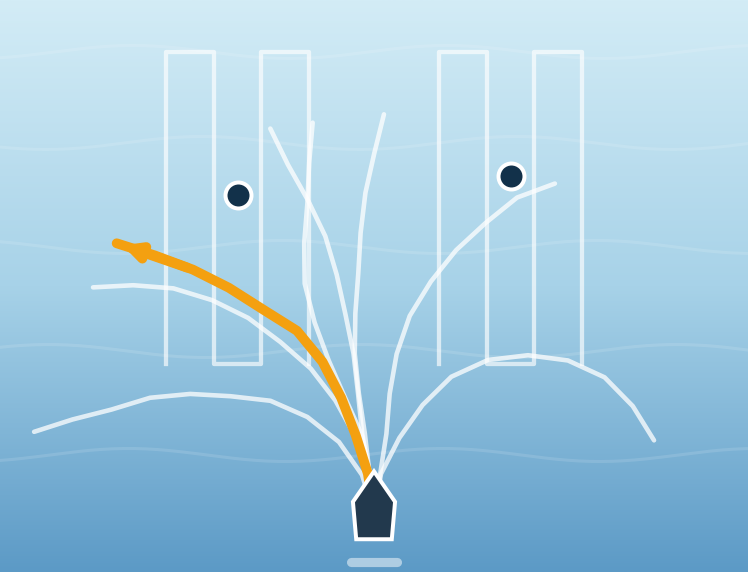
\includegraphics[width=0.42\textwidth]{Trajectory Generation.png}
\caption{Trajectory generation: from its current pose the ASV samples many candidate paths and commits the
cost-weighted one toward the survey.}
\label{fig:trajgen}
\end{figure}

\section{Low-level control and acoustic exchange}
The committed reference is tracked by a lookahead waypoint follower with proportional--derivative steering,
producing the two thruster commands $(f_L,f_R)$ of the Otter surface vehicle. When a ping is issued the ASV
emits an interrogation pulse; the AUV's transponder replies; the USBL measures range (round-trip time) and
bearing (array phase) and forms the three-dimensional fix, which is then applied to the AUV filter as an
OOSM (\secref{sec:usblmodel}). Only one such exchange occurs per slot.

% ============================================================================
\chapter{Simulation Setup and Metrics}
\label{ch:setup}

\section{Simulator}
The study uses a marine-vehicle simulator built on standard hydrodynamic models \cite{fossen2011handbook}:
a REMUS-class AUV and an Otter surface craft, with an acoustic model that reproduces the finite speed of
sound, the two-way travel-time delay, and the resulting out-of-sequence fixes. The AUVs steer on their own
(estimate-fed) navigation; no ground truth is used in any control or planning decision.

\section{Scenario and configuration}
Two AUVs run laterally separated vertical lawnmower surveys, each leg $200$\,m long, at $40$\,m depth, while
one ASV supports both over a $500$\,m-rated USBL link. \tabref{tab:config} lists the main settings and
\figref{fig:geom} shows the geometry; the full parameter list is in Appendix~\ref{app:params}.

\begin{table}[H]
\centering
\caption{Main simulation configuration.}
\label{tab:config}
\begin{tabular}{@{}ll@{}}
\toprule
Parameter & Value \\
\midrule
Number of AUVs & 2 \\
Lawnmower leg length & 200\,m \\
Lateral AUV separation & 260\,m \\
AUV survey depth & 40\,m \\
USBL rated range $R_{\text{oper}}$ & 500\,m \\
Ping slot cadence $T_{\text{slot}}$ & 1.3\,s \\
Safeguard interval $T_{\text{safe}}$ & 15\,s \\
Covariance trigger $\tau_{\text{trig}}$ & 20\,m$^2$ \\
Coverage weight $w_{\text{cov}}$ & 400 \\
MPPI rollouts $K$ & 192 \\
USBL range / bearing noise & 0.10\,m / $0.5^{\circ}$ \\
ASV position noise $\sigma_{\text{gps}}$ & 1.0\,m \\
Speed of sound & 1500\,m$\,$s$^{-1}$ \\
\bottomrule
\end{tabular}
\end{table}

\begin{figure}[H]
\centering
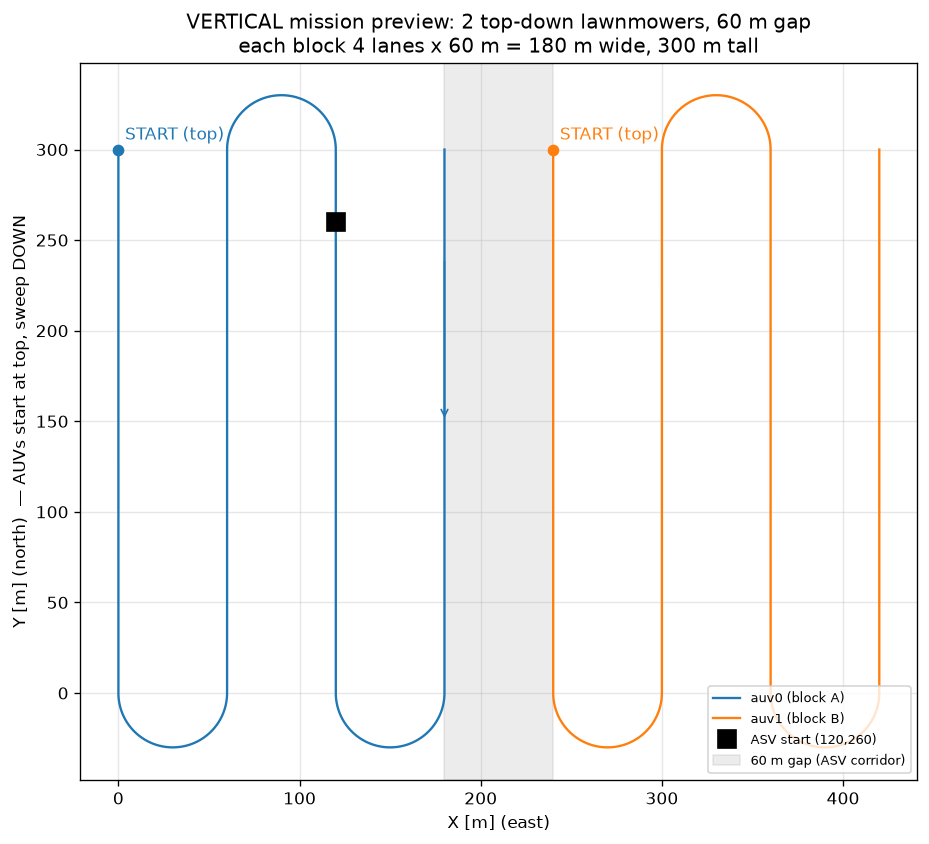
\includegraphics[width=0.7\textwidth]{survey_geometry.png}
\caption{The two-AUV lawnmower survey and the ASV support geometry.}
\label{fig:geom}
\end{figure}

\section{Evaluation metrics}
\begin{description}
\item[True / estimated cross-track error.] Perpendicular distance of the AUV's true (resp.\ estimated)
position from its planned lane; the primary survey-accuracy measure.
\item[EKF horizontal error.] $\lVert(\hat{x},\hat{y})-(x,y)_{\text{true}}\rVert$, the filter's actual
horizontal error.
\item[Fixes delivered / lost.] Number of USBL fixes delivered, and how many were lost to range or channel.
\item[Consistency (ANEES).] Average normalised estimation error squared; near $1$ indicates the reported
covariance matches the true error \cite{barshalom2001estimation}.
\item[Maximum slant range.] Largest ASV--AUV distance, relative to the $500$\,m envelope.
\end{description}

% ============================================================================
\chapter{Results}
\label{ch:results}

\section{Why acoustic aiding is needed: a feasibility progression}
\label{sec:feasibility}
Two reference points establish why in-situ acoustic aiding is necessary. \tabref{tab:progression} places
three navigation approaches side by side. \textbf{These are different navigation paradigms on a different
survey geometry (a shared box), not a like-for-like benchmark;} they are shown as an order-of-magnitude
feasibility progression, and the cited figures are structural ones that do not depend on the geometry.

\begin{table}[H]
\centering
\caption{Feasibility progression (order-of-magnitude; different operating conditions, \emph{not} a
controlled benchmark).}
\label{tab:progression}
\begin{tabular}{@{}p{3.4cm}p{3.0cm}p{3.4cm}p{3.2cm}@{}}
\toprule
Approach & Aiding & Accuracy / drift & Outcome \\
\midrule
Unaided inertial navigation & none & budget (4.47\,m) exceeded in \textbf{$\sim$12\,s}; drift grows to
$\sim$10$^6$\,m & survey never completes \\
Periodic surfacing for GPS + depth sensor (at 40\,m) & intermittent surface GPS; depth sensor (vertical
only) & between-fix error km-scale; true coverage $\sim$21\% & impractical ($\sim$32\% survey duty) \\
\textbf{ASV + USBL planner (this work)} & in-situ acoustic USBL & true cross-track $\sim$\textbf{2\,m};
0 fixes lost & full survey completed \\
\bottomrule
\end{tabular}
\end{table}

\paragraph{Unaided inertial navigation.} With zero measurement updates, the filter's own covariance crosses
the $4.47$\,m budget in $12.2$\,s for both AUVs; the trajectory then diverges to order $10^{6}$\,m and the
survey never completes. This $12.2$\,s figure is robust across configurations---it happens early, before
chaotic amplification---so it is a structural property of the IMU, not of a particular mission.

\paragraph{Periodic surfacing for GPS.} A vehicle that periodically surfaces for a GPS fix (with a pressure
sensor aiding only the vertical channel) is bounded in depth but not horizontally: at a $40$\,m survey depth
the climb-and-dive round trip is so slow that the horizontal error grows to kilometre scale between fixes
and true coverage is only about $21\%$. A depth sweep confirms the trend---between-fix error falls from
$\sim$21\,km at $40$\,m to $\sim$55\,m at $3$\,m and coverage rises to $78\%$---but even at $3$\,m (not a
realistic survey depth) the vehicle surveys only about a third of the time and the residual error is worse
than a single acoustic fix would give. Surfacing is therefore impractical, which motivates in-situ acoustic
aiding.

\section{Planner performance}
\label{sec:perf}
\tabref{tab:results} summarises a full survey run with the ASV + USBL planner. Both AUVs are held to a true
cross-track error of about $2$\,m (95th percentile near $5$\,m); the maximum ASV--AUV slant range stays well
inside the $500$\,m envelope; and \emph{every} acoustic fix requested is delivered---none is lost to range.
The navigation covariance is statistically consistent (ANEES close to $1$). \figref{fig:results} and
\figref{fig:results3d} show the AUV and ASV tracks.

\begin{table}[H]
\centering
\caption{Per-AUV results for a full two-AUV survey run with the ASV + USBL planner.}
\label{tab:results}
\begin{tabular}{@{}lcc@{}}
\toprule
Metric & AUV\,0 & AUV\,1 \\
\midrule
True cross-track error, mean & 1.98\,m & 1.86\,m \\
True cross-track error, 95th pct.\ & 5.58\,m & 4.80\,m \\
EKF horizontal error, mean & 1.78\,m & 1.73\,m \\
Fixes delivered & 320 & 319 \\
Max ASV--AUV slant range & 172\,m & 186\,m \\
Range-limited losses & 0 & 0 \\
Covariance consistency (ANEES) & 1.01 & 0.81 \\
Heading error (RMS) & $5.4^{\circ}$ & $4.8^{\circ}$ \\
\bottomrule
\end{tabular}
\end{table}

\noindent Across the fleet the USBL delivered all $639$ requested pings with $0$ lost, and the mission was
flagged safe (no range violations). The ASV covered $2298$\,m at a mean speed of $2.74$\,m$\,$s$^{-1}$ while
serving both vehicles; both AUVs completed their surveys in about $838$\,s.

\begin{figure}[htbp]
\centering
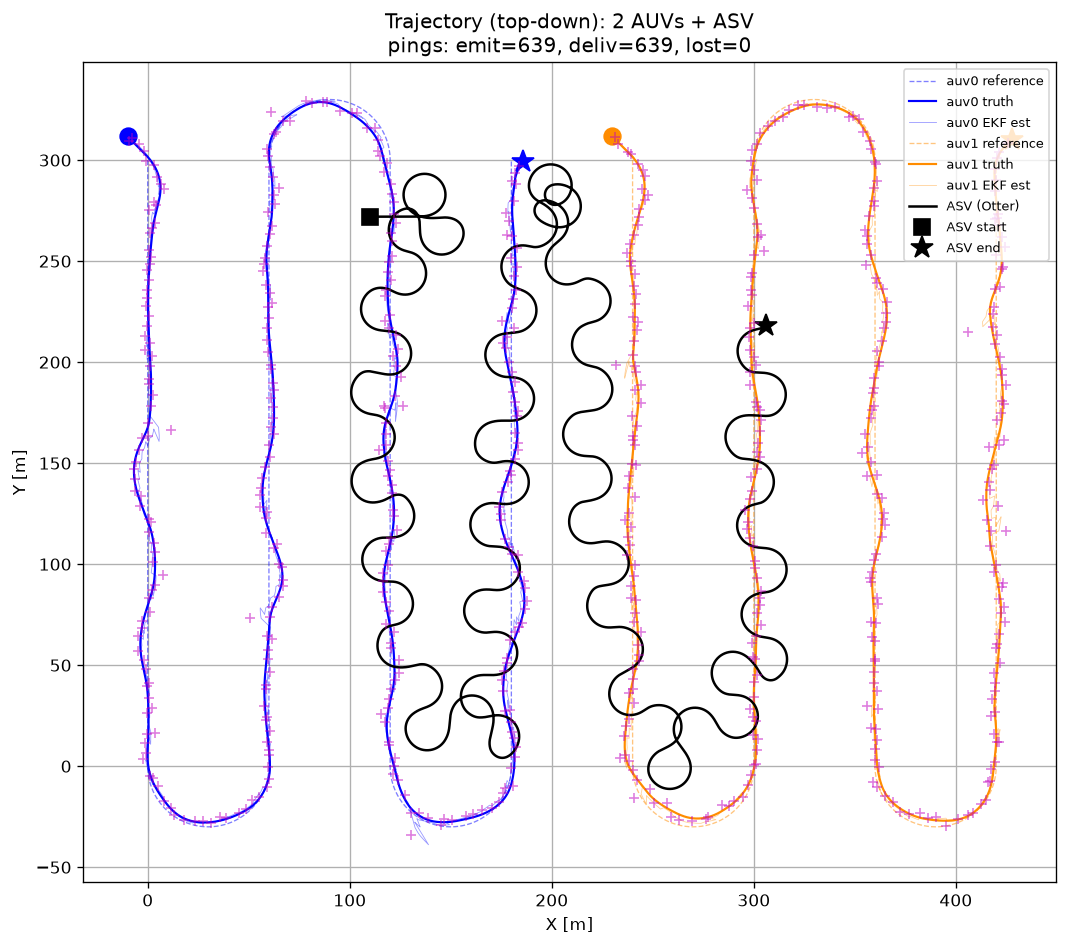
\includegraphics[width=0.48\textwidth]{results_traj2d.png}\hfill
\caption{ AUV survey tracks and the ASV path (top-down)}
\label{fig:results}
\end{figure}

\begin{figure}[H]
\centering
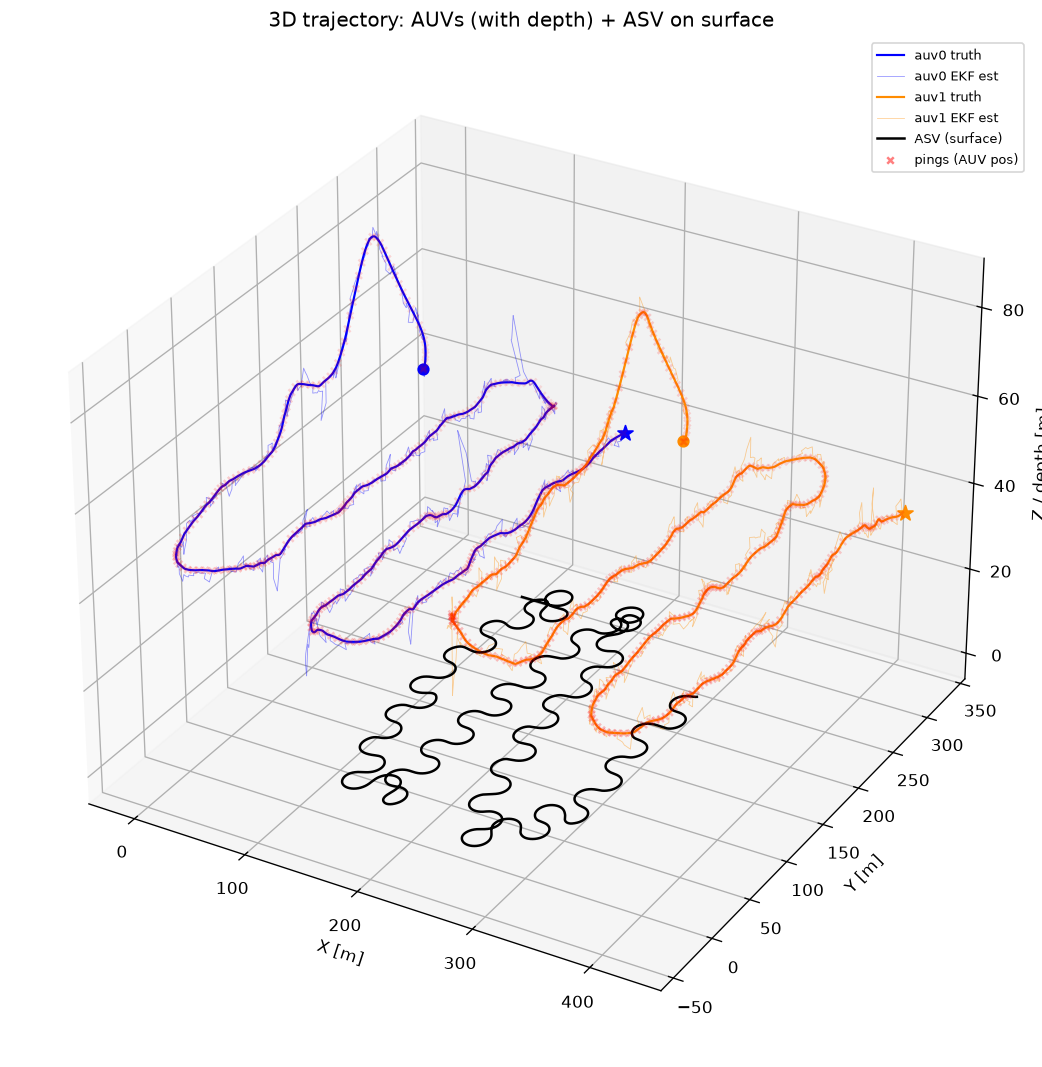
\includegraphics[width=0.6\textwidth]{results_traj3d.png}
\caption{Three-dimensional view of the two AUV survey tracks and the surface ASV, showing the fleet held
within the acoustic envelope throughout the mission.}
\label{fig:results3d}
\end{figure}

Where the unaided navigator diverges in seconds and periodic surfacing leaves kilometre-scale gaps at survey
depth, the acoustic-aided planner holds both AUVs near $2$\,m for the entire mission while never losing a
fix. The consistency check (ANEES $\approx 1$) confirms the covariance the trigger relies on is honest.

\section{Positioning strategy: MPPI versus a centroid baseline}
\label{sec:mppivscentroid}
To isolate the value of the MPPI \emph{positioning} (as distinct from the trigger and cost), the same
mission was run with the MPPI planner replaced by a trivial baseline that steers the ASV straight to the
fleet centroid each slot. \tabref{tab:mppivscentroid} compares them: both keep the fleet accurate
($\sim2$\,m true cross-track) and lose \emph{no} fixes, but the centroid baseline does so with markedly less
ASV travel ($1467$\,m versus $2298$\,m) and a lower mean speed. In this comfortably-in-range geometry the
MPPI positioning therefore does not improve accuracy or coverage over the simple centroid; its value would
be expected only where geometry is tighter or the fleet more spread.

\begin{table}[H]
\centering
\caption{MPPI positioning versus the centroid baseline, same two-AUV mission.}
\label{tab:mppivscentroid}
\begin{tabular}{@{}lccc@{}}
\toprule
Metric & MPPI & Centroid \\
\midrule
True cross-track (AUV\,0 / AUV\,1), mean & 1.98 / 1.86\,m & 1.94 / 1.81\,m \\
Fixes delivered / lost & 639 / 0 & 638 / 0 \\
Max slant range (AUV\,0 / AUV\,1) & 172 / 186\,m & 147 / 154\,m \\
ASV path length & 2298\,m & 1467\,m \\
ASV mean speed & 2.74\,m$\,$s$^{-1}$ & 1.75\,m$\,$s$^{-1}$ \\
\bottomrule
\end{tabular}
\end{table}

\section{The range envelope: an out-of-range capacity limit}
\label{sec:outofrange}
The results above assume both AUVs stay within the USBL envelope. \tabref{tab:outofrange} stretches the
lateral separation so the fleet approaches and then exceeds the $500$\,m reach. As the maximum slant range
climbs past the envelope, fixes begin to be lost and the \emph{true} cross-track error grows explosively---
from $\sim2$\,m in range to tens and then hundreds of metres---while the AUVs' \emph{own} estimate stays
small (they are, in effect, confidently lost). Neither the MPPI planner nor the centroid recovers: with the
AUVs on opposite sides of a wide corridor a single ASV cannot be within range of both at once. This is a
\emph{capacity/geometry} limit, not a control deficiency; the remedies are additional ASVs or a bounded
survey geometry, not a smarter cost.

\begin{table}[H]
\centering
\caption{Effect of widening the AUV separation (all with the same planner). ``COMMS-LOSS'' marks runs where
the fleet left the USBL envelope. True cross-track is the AUV's actual error; its \emph{estimated}
cross-track stays near $1.5$--$5$\,m throughout.}
\label{tab:outofrange}
\begin{tabular}{@{}lcccc@{}}
\toprule
Case & Planner & Max slant & Fixes lost & True cross-track (AUV\,0 / AUV\,1) \\
\midrule
In-range control      & MPPI     & 256--280\,m & 0   & 1.80 / 1.69\,m \\
Wide (gap $\approx500$\,m) & MPPI     & 471--484\,m & 58  & 1.70 / 1.42\,m \\
Wide (gap $\approx500$\,m) & Centroid & 442--463\,m & 29  & 1.97 / 1.81\,m \\
Out of range          & MPPI     & 577--850\,m & 635 & 32.9 / 17.1\,m \\
Out of range          & Centroid & 671--1061\,m & 636 & 65.7 / 34.8\,m \\
\bottomrule
\end{tabular}
\end{table}

% ============================================================================
\chapter{Analysis and Discussion}
\label{ch:analysis}

\section{Roles of the cost terms}
The cost \eqnref{eq:cost} combines terms that play distinct roles, which is clearest when they are read
against the mission. \emph{Coverage} is the \emph{reachability} driver: its heavy weight makes it dominate
whenever an AUV nears the edge of the USBL range, so the ASV first and foremost keeps every vehicle
pingable. \emph{Information gain} is the \emph{fix-quality} driver: among positions that are all reachable,
it prefers geometries where the next fix would most reduce an AUV's uncertainty, and its staleness discount
favours nearer (faster) fixes. The \emph{control-effort} penalties merely damp needless turning and speed.
In the surveyed regime the coverage term does most of the work---the fleet is always comfortably in range
(max slant $\le186$\,m against a $500$\,m envelope), so reachability, not fix geometry, sets where the ASV
goes.

\section{The cost landscape}
\label{sec:landscape}
To see \emph{why} coverage dominates, the position-cost was sampled on a grid around the fleet at a fixed
instant. The total cost is a \emph{flat-bottomed bowl} centred on the fleet centroid: it varies only weakly
over the reachable region and then rises steeply as the AUVs near the range edge. Decomposed, the coverage
term is a single centring bowl pulling the ASV toward the fleet mid-point, while the information-gain term is
a much weaker, bimodal ripple (a shallow well near each AUV). The near-flat bottom of this landscape is the
root of the residual-motion issue discussed in \secref{sec:wobble}: near the optimum the cost provides
almost no gradient, so the planner has little to lock onto.

\section{Cost-term ablations}
\label{sec:ablations}
The role of each cost term was probed by removing or sweeping it (\tabref{tab:ablation}). The starting point
for these sweeps is a reduced-cost variant of the planner, so the figures are internal to each sweep rather
than directly comparable to the full-system run of \chapref{ch:results}; all are in range unless noted, and
none of the levers recovered the out-of-range failure of \secref{sec:outofrange}.

\begin{table}[H]
\centering
\caption{Cost-term ablations (in-range). ``ASV path'' is the surface vehicle's travelled distance, a proxy
for how much it roams; accuracy stayed near $2$\,m throughout unless stated.}
\label{tab:ablation}
\begin{tabular}{@{}p{4.3cm}p{2.3cm}p{2.4cm}p{4.0cm}@{}}
\toprule
Lever (swept) & Fixes lost & ASV path & Effect \\
\midrule
Coverage removed (information-gain only) & 3 (in) / 455 (out) & 1827\,m &
The ASV neglects one AUV (its slant grows to $464$\,m); out of range it collapses (only $2$ fixes). Coverage
is the reachability driver. \\
Energy penalty $R_v$: $0\!\to\!0.5\!\to\!2$ & 0 & $1826\!\to\!924$\,m &
Roaming halves as the ASV parks near the fleet; accuracy unchanged. \\
Turn penalty $R_\omega$: $0\!\to\!20$ & 0 & $924$\,m (flat) &
No further change---the residual motion is not driven by this penalty. \\
Direction-flip penalty: $0\!\to\!2000$ & 0 & $1639\!\to\!1381$\,m &
Penalising steering reversals trims roaming modestly, then saturates. \\
Coverage\,$\times$\,jerk grid & 0 & $\sim1600$--$1650$\,m &
Adding a jerk penalty barely moves the ASV travel. \\
Reference-tracking weight: $0\!\to\!6400$ & 0 & $1639\!\to\!1354$\,m &
Stronger tracking of a straight reference gently reduces roaming. \\
Command low-pass filter: $\tau\,0\!\to\!5$ & 0 & $1639\!\to\!1721$\,m &
Low-passing the command does \emph{not} reduce roaming. \\
Predictive pre-positioning (on/off) & $103\!\to\!98$; $681\!\to\!672$ & $\sim2400$\,m &
Negligible: it redistributes fixes but adds no capacity. \\
Station-keeping heading-hold (off/on) & 0 & $924\!\to\!67$\,m &
The ASV parks almost completely yet still delivers every fix (in range). \\
\bottomrule
\end{tabular}
\end{table}

\noindent The consistent picture is that \emph{coverage} sets reachability, an \emph{energy/settle} term
controls how much the ASV roams, and no single penalty on turning, jerk, or command smoothness removes the
residual motion---foreshadowing \secref{sec:wobble}.

\section{Information geometry of the fix}
\label{sec:infogeom}
The value of the information-gain term depends on the \emph{shape} of the prior covariance it is scored
against. Holding an AUV's predicted position and total uncertainty fixed and varying only the ASV's approach
bearing, the $D$-optimal gain \eqnref{eq:gamma} was evaluated on a circle around the AUV.

With an \emph{isotropic} prior the gain is \textbf{independent of bearing} (spread $\approx0\%$): the
measurement information $\mathbf{J}$ is anisotropic (precise in range, coarse across it), but a round prior
makes the $D$-optimal score rotation-invariant, so the geometry term carries no directional signal. With a
path-frame \emph{ellipse} prior of the same total uncertainty the gain varies markedly with bearing (spread
rising into the tens of percent as the ellipse is elongated), with a well-defined preferred approach
direction (\figref{fig:infogain}).

\begin{figure}[htbp]
\centering
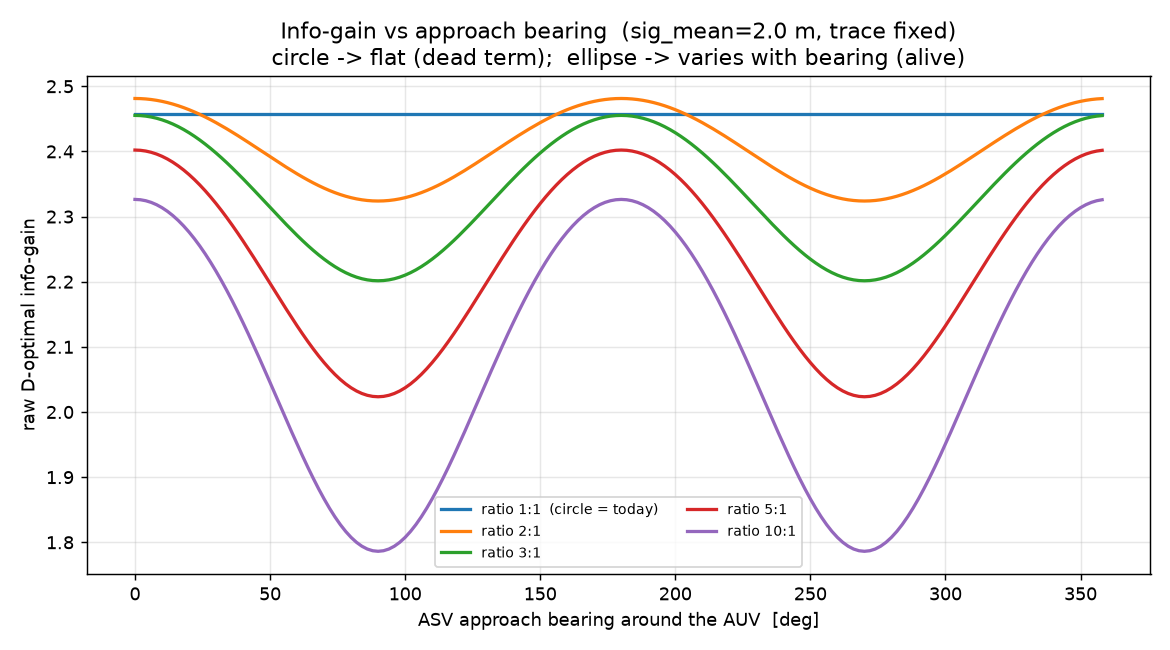
\includegraphics[width=0.7\textwidth]{infogain_vs_bearing.png}
\caption{Information gain versus ASV approach bearing for priors of equal total uncertainty but different
shape. A circular prior gives a flat (bearing-independent) gain; an elongated ellipse gives a clear
preferred bearing.}
\label{fig:infogain}
\end{figure}

However, replacing the planner's prior with the elongated ellipse in the \emph{full} mission changed the
outcome negligibly: cross-track, fixes and losses were identical to the isotropic case (all $639$ fixes
delivered, $0$ lost). The reason follows from \secref{sec:infogeom} above---in this regime the heavily
weighted coverage term dominates the cost, so reviving the geometry term's bearing sensitivity does not, by
itself, change where the ASV goes. The geometry term is a genuine, principled component, but its influence
is latent behind coverage at the operating point studied.

\section{Motion smoothness: localising the residual wobble}
\label{sec:smoothness}
The ASV's cruise motion carries a persistent low-amplitude wobble. To localise its cause, the total heading
turned by the executed ASV path over a full mission was used as a smoothness metric, and three interventions
were swept (\tabref{tab:wobble}); throughout, accuracy and fixes were essentially unchanged
($\sim639$ delivered, $0$ lost, $\sim2$\,m cross-track), so the interventions do no harm---they simply fail
to help.

\begin{table}[H]
\centering
\caption{Total heading turned by the executed ASV path (lower is smoother) under three interventions. The
analytic centroid controller is included as a smoothness reference.}
\label{tab:wobble}
\begin{tabular}{@{}ll@{}}
\toprule
Intervention & Total heading turned \\
\midrule
Baseline MPPI & $11601^{\circ}$ \\
Controller heading low-pass ($\alpha=0.15$ / $0.03$) & $11611^{\circ}$ / $11108^{\circ}$ \\
Colored-noise sampling ($\rho=0.7$ / $0.9$) & $12079^{\circ}$ / $12112^{\circ}$ \\
Steep-cost well ($6\times$ / $60\times$ the coverage bowl) & $11398^{\circ}$ / $10619^{\circ}$ \\
Analytic centroid controller (no sampling) & $1735^{\circ}$ \\
\bottomrule
\end{tabular}
\end{table}

\noindent No intervention \emph{inside} the sampling planner removes the wobble: low-passing the heading is
inert, colored-noise sampling is slightly worse, and even a $60\times$ steeper cost trims the turning by only
$\sim8\%$ (while increasing steering reversals, because a strong attractor makes the moving ASV orbit the
target). The one smooth controller---the analytic centroid, which uses \emph{no} sampling and settles rather
than orbits---turns $6.7\times$ less. This localises the cause: as \secref{sec:landscape} showed, the cost is
nearly flat at its optimum, so the MPPI softmax weights stay near-uniform and the committed control is
dominated by residual sampling noise; the minimum-speed constraint then forces continual motion around the
target. The wobble is therefore intrinsic to the sampling planner on a flat cost, and the appropriate remedy
is a non-sampling or settle-capable controller (\secref{sec:wobble}).

% ============================================================================
\chapter{Conclusion, Limitations and Future Work}
\label{ch:conclusion}

This report described an ASV positioning planner for acoustic-aided AUV localisation. The ASV maintains an
uplink-free shadow of each AUV's position and uncertainty, triggers a USBL fix when that uncertainty crosses
a threshold, selects which AUV to serve under a half-duplex constraint, and steers itself with an MPPI
planner whose cost trades fix information gain against keeping the fleet in range. In simulation the planner
keeps two surveying AUVs inside the acoustic envelope, delivers every requested fix, and holds the true
cross-track error near $2$\,m with statistically consistent uncertainty---where an unaided navigator would
diverge within seconds and periodic surfacing would be impractical at survey depth.

\section{Open issue: residual ASV motion}
\label{sec:wobble}
The one unresolved issue is a persistent low-amplitude \emph{wobble} in the ASV's cruise motion. Its cause
is intrinsic to the sampling planner: on a cost that is locally flat near its optimum, the MPPI softmax
weights \eqnref{eq:mppiw} stay nearly uniform, so the committed control is dominated by the residual mean of
the sampled noise---a small, randomly-changing turn command every slot---rather than by a clear gradient. A
minimum-speed constraint (the ASV cannot stop) compounds this by forcing motion \emph{around} a target
rather than settling on it.

Three interventions were tried and \emph{none} removed the wobble, which localises the cause rather than
fixing it: (i) low-pass filtering the desired heading at the controller layer changed the total executed
turning only marginally; (ii) sampling temporally-correlated (colored) control noise did not reduce it;
and (iii) steepening the cost with a quadratic well at the fleet centroid---up to $60\times$ the coverage
bowl---moved the total executed turning only from $11601^{\circ}$ to $10619^{\circ}$ while \emph{increasing}
the number of steering reversals, because a strong attractor makes the moving ASV orbit the target. These
results indicate that the wobble cannot be filtered or cost-shaped away within the sampling planner; a
non-sampling (analytic) or explicitly settle-capable controller is the appropriate remedy, and is left as
future work.

\section{Other limitations and future work}
The reported results are from a single survey geometry and a single random seed; a broader study over fleet
size, separation, depth and sea state remains to be done, ideally as a Monte-Carlo evaluation with
confidence intervals and controlled, same-mission comparisons of each design choice. When a single ASV must
serve AUVs that are far apart, keeping all of them in range becomes a capacity/geometry limit that no
positioning strategy can overcome; additional ASVs or bounded geometry are then required. Finally, a future
navigator that fuses an additional asynchronous velocity measurement would benefit from an error-state
(ESKF) covariance formulation, which handles rotation uncertainty and delayed measurements more cleanly than
the direct Euler-angle EKF used here.

% ============================================================================
\appendix
\chapter{Full Parameter List}
\label{app:params}
\begin{table}[H]
\centering
\caption{Simulation and planner parameters.}
\begin{tabular}{@{}lll@{}}
\toprule
Group & Parameter & Value \\
\midrule
Timing        & integration step $\Delta t$ & 0.02\,s (50\,Hz) \\
              & ping slot $T_{\text{slot}}$ & 1.3\,s \\
              & safeguard $T_{\text{safe}}$ & 15\,s \\
Geometry      & AUVs & 2 \\
              & leg length & 200\,m \\
              & lateral separation & 260\,m \\
              & lane spacing & 60\,m \\
              & turn radius & 30\,m \\
              & survey depth & 40\,m \\
              & depth profile & $\pm$3\,m, 75\,s period \\
AUV speed     & cruise & 1.0\,m$\,$s$^{-1}$ \\
USBL          & rated range & 500\,m \\
              & range noise $\sigma_r$ & 0.10\,m \\
              & bearing noise $\sigma_a$ & $0.5^{\circ}$ \\
              & ASV position noise $\sigma_{\text{gps}}$ & 1.0\,m \\
              & speed of sound & 1500\,m$\,$s$^{-1}$ \\
Trigger       & $\tau_{\text{trig}}$ & 20\,m$^2$ \\
MPPI          & rollouts $K$ & 192 \\
              & turn-rate / speed noise & 0.12 / 0.7 \\
              & temperature $\lambda$ & 1.0 \\
              & max turn rate $\omega_{\max}$ & 0.85\,rad$\,$s$^{-1}$ \\
              & speed range $[v_{\min},v_{\max}]$ & $[1.0,\,3.0]$\,m$\,$s$^{-1}$ \\
              & turn / energy penalty $R_\omega,R_v$ & 0.10 / 0 \\
Cost          & coverage weight $w_{\text{cov}}$ & 400 \\
Aids          & gravity levelling, COG heading & enabled \\
\bottomrule
\end{tabular}
\end{table}
\noindent Initial and process covariances $\mathbf{P}_0,\mathbf{Q}$ are diagonal, derived from the IMU
specification (an EuRoC / ADIS16448-class MEMS IMU); their exact entries are set in the simulation source.

\chapter{Derivations}
\label{app:deriv}
The derivations below are given in dependency order: the propagation Jacobian $\mathbf{F}$ from the
strapdown equations; the USBL information matrix $\mathbf{J}$ from the geometry; the information gain
$\Gamma$; the EKF measurement update; and the out-of-sequence procedure.

\section{The state-transition Jacobian $\mathbf{F}$}
\label{app:F}
$\mathbf{F}=\partial\mathbf{x}^{+}/\partial\mathbf{x}$ is obtained by differentiating the propagation
\eqnref{eq:rot}--\eqnref{eq:vz} entry by entry; $\mathbf{F}=\mathbf{I}$ plus the couplings below (writing
$c=\cos\psi$, $s=\sin\psi$; the small factor $\lambda\approx1$).

\emph{Position from velocity.} From \eqnref{eq:pos} and \eqnref{eq:psiz},
$\partial x^{+}/\partial v_x=\partial y^{+}/\partial v_y=\partial z^{+}/\partial v_z=\Delta t$.

\emph{Velocity self-damping.} From \eqnref{eq:vel},\,\eqnref{eq:vz},
$\partial v_x^{+}/\partial v_x=\partial v_y^{+}/\partial v_y=\partial v_z^{+}/\partial v_z=\lambda$.

\emph{Heading from gyro bias.} The de-biased yaw rate is $r^c=\omega_z-b_{gz}$, so from \eqnref{eq:psiz}
$\partial \psi^{+}/\partial b_{gz}=-\Delta t$.

\emph{Velocity from heading.} The world-frame acceleration \eqnref{eq:rot} depends on $\psi$ through $c,s$.
Differentiating, $\partial a_x^w/\partial\psi=-s\,a_x^c-c\,a_y^c=-a_y^w$ and
$\partial a_y^w/\partial\psi=c\,a_x^c-s\,a_y^c=a_x^w$. Hence, via \eqnref{eq:vel},
\begin{equation}
\frac{\partial v_x^{+}}{\partial \psi}=-\lambda\,a_y^w\,\Delta t,\qquad
\frac{\partial v_y^{+}}{\partial \psi}= \lambda\,a_x^w\,\Delta t .
\end{equation}
This coupling is what lets a heading error inflate the horizontal velocity (and thence position) uncertainty.

\emph{Velocity from accelerometer bias.} With $a_x^c=a_x^{\text{kin}}-b_{ax}$, $a_y^c=a_y^{\text{kin}}-b_{ay}$
and \eqnref{eq:rot}, $\partial a_x^w/\partial b_{ax}=-c$, $\partial a_x^w/\partial b_{ay}=s$,
$\partial a_y^w/\partial b_{ax}=-s$, $\partial a_y^w/\partial b_{ay}=-c$. Therefore
\begin{equation}
\frac{\partial v_x^{+}}{\partial b_{ax}}=-\lambda c\,\Delta t,\;\;
\frac{\partial v_x^{+}}{\partial b_{ay}}= \lambda s\,\Delta t,\;\;
\frac{\partial v_y^{+}}{\partial b_{ax}}=-\lambda s\,\Delta t,\;\;
\frac{\partial v_y^{+}}{\partial b_{ay}}=-\lambda c\,\Delta t,\;\;
\frac{\partial v_z^{+}}{\partial b_{az}}=-\lambda\,\Delta t .
\end{equation}
The corresponding position couplings are the second-order terms
$\partial x^{+}/\partial b_{ax}=-\tfrac12 c\,\Delta t^{2}$, etc., from the $\tfrac12 a^w\Delta t^2$ term in
\eqnref{eq:pos}. Roll and pitch $(\phi,\theta)$ propagate by the analogous Euler-rate relations and are
corrected by gravity levelling; on the near-level survey legs their coupling into the horizontal states is
small. The COG aid \eqnref{eq:cog} has scalar Jacobian $\partial c_{\text{cog}}/\partial\psi=1$,
$\partial c_{\text{cog}}/\partial v_x=v_y/(v_x^2+v_y^2)$, $\partial c_{\text{cog}}/\partial v_y=-v_x/(v_x^2+v_y^2)$.

\section{The USBL information matrix $\mathbf{J}$}
\label{app:J}
Let the ASV be at $(x_a,y_a)$ and the (predicted) AUV at $(x_u,y_u,z_u)$, with $dx=x_u-x_a$, $dy=y_u-y_a$,
$dz=z_u$, horizontal range $h=\sqrt{dx^2+dy^2}$, slant range $sl=\sqrt{h^2+dz^2}$, bearing
$brg=\operatorname{atan2}(dy,dx)$ and elevation with $\sin z=h/sl$. The transceiver measures range with
standard deviation $\sigma_r$ and bearing with angular standard deviation $\sigma_a$; a bearing error maps
to a cross-range position error $\sigma_{\text{ang}}=sl\,\sigma_a/\sin z$ (it grows with range). In a frame
aligned with the line of sight the horizontal measurement covariance is therefore diagonal,
$\boldsymbol{\Lambda}=\operatorname{diag}(\sigma_r^2,\sigma_{\text{ang}}^2)$ (precise along range, coarse
across it). Rotating this into world axes by the bearing $brg$ with
$\mathbf{V}=\left[\begin{smallmatrix}\cos brg&-\sin brg\\ \sin brg&\cos brg\end{smallmatrix}\right]$, and
adding the ASV's own (isotropic) position uncertainty $\sigma_{\text{gps}}^2\mathbf{I}$, gives
$\mathbf{R}_m=\mathbf{V}\boldsymbol{\Lambda}\mathbf{V}^{\!\top}+\sigma_{\text{gps}}^2\mathbf{I}$, and the
information the fix contributes is its inverse $\mathbf{J}=\mathbf{R}_m^{-1}$ \eqnref{eq:jmeas}. The
anisotropy of $\mathbf{J}$ (its dependence on $brg$) is exactly the directional signal analysed in
\secref{sec:infogeom}.

\section{The information gain $\Gamma$}
\label{app:gamma}
Let $\mathbf{P}_{\text{fut}}$ be the AUV's predicted position covariance at the instant the (delayed) fix
would land, i.e.\ the shadow covariance propagated forward by the round-trip delay $d$ using
\eqnref{eq:covprop}. Fusing a measurement of information $\mathbf{J}$ combines two independent Gaussian
sources, which in information form add:
$\mathbf{P}_{\text{post}}^{-1}=\mathbf{P}_{\text{fut}}^{-1}+\mathbf{J}$, hence
$\mathbf{P}_{\text{post}}=(\mathbf{P}_{\text{fut}}^{-1}+\mathbf{J})^{-1}$. Under the $D$-optimality
criterion the ``size'' of an uncertainty is the log-volume of its covariance ellipsoid,
$\tfrac12\log\det\mathbf{P}$ up to a constant, so the information gained by the fix is the reduction
\begin{equation}
\log\det\mathbf{P}_{\text{fut}}-\log\det\mathbf{P}_{\text{post}}
=\log\det\!\big(\mathbf{I}+\mathbf{P}_{\text{fut}}\mathbf{J}\big)\;\ge 0 .
\end{equation}
Multiplying by the staleness discount $e^{-\lambda_s d}$ (a fix that takes longer to arrive is worth less)
and subtracting the constant expected communication cost $p_{\text{comm}}$ gives $\Gamma$ in
\eqnref{eq:gamma}. Because $p_{\text{comm}}$ is constant it shifts every candidate's score equally and does
not affect \emph{which} position is preferred; the spatial signal lives in $\mathbf{J}$ (via geometry) and
in $d$ (via slant range).

\section{The EKF measurement update}
\label{app:upd}
For a linear(ised) measurement $\mathbf{z}=\mathbf{H}\mathbf{x}+\mathbf{v}$, $\mathbf{v}\sim(0,\mathbf{R})$,
with prior $\mathbf{x}\sim(\hat{\mathbf{x}},\mathbf{P})$, the innovation is
$\boldsymbol{\nu}=\mathbf{z}-\mathbf{H}\hat{\mathbf{x}}$ with covariance
$\mathbf{S}=\mathbf{H}\mathbf{P}\mathbf{H}^{\!\top}+\mathbf{R}$. Seeking a linear corrector
$\hat{\mathbf{x}}^{+}=\hat{\mathbf{x}}+\mathbf{K}\boldsymbol{\nu}$ that minimises the posterior error
covariance trace, the posterior (Joseph form) is
$\mathbf{P}^{+}=(\mathbf{I}-\mathbf{K}\mathbf{H})\mathbf{P}(\mathbf{I}-\mathbf{K}\mathbf{H})^{\!\top}
+\mathbf{K}\mathbf{R}\mathbf{K}^{\!\top}$; setting
$\partial\operatorname{tr}\mathbf{P}^{+}/\partial\mathbf{K}=0$ gives the Kalman gain
$\mathbf{K}=\mathbf{P}\mathbf{H}^{\!\top}\mathbf{S}^{-1}$, whereupon
$\mathbf{P}^{+}=(\mathbf{I}-\mathbf{K}\mathbf{H})\mathbf{P}$ \cite{barshalom2001estimation}. This is
\eqnref{eq:usblupdate}; the USBL $\mathbf{H}$ selects the three position states, the gravity-levelling and
COG aids use the scalar/low-dimensional $\mathbf{H}$ of Appendix~\ref{app:F}.

\section{Out-of-sequence fusion (OOSM)}
\label{app:oosm}
A USBL fix is valid at the instant $t_{\text{valid}}$ the interrogation reaches the AUV, but only arrives at
$t_{\text{arrive}}=t_{\text{valid}}+\text{(return + processing delay)}$, by which time the filter has
propagated past it. Fusing at the arrival time would apply the measurement against a mismatched state. The
filter therefore keeps a bounded history of $(t,\mathbf{x},\mathbf{P},\text{IMU})$ and, on arrival: (1) if
$t_{\text{valid}}$ is older than the history, discards the fix; (2) otherwise rewinds $\mathbf{x},\mathbf{P}$
to the stored entry nearest $t_{\text{valid}}$; (3) applies the update of Appendix~\ref{app:upd} there; and
(4) re-propagates (\emph{replays}) the stored IMU samples from that instant forward to the present. The fix
thus corrects the state at the time it was actually valid, and the correction is carried forward
consistently through the intervening motion.

\printbibliography[heading=bibintoc]

\end{document}
